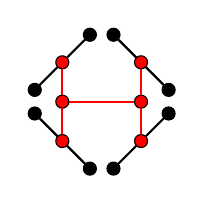
\begin{tikzpicture}[auto,scale=0.5]

	\node (c0) [circle, draw, fill=red, scale=0.5] at (0, 0) {};
	\node (c1) [circle, draw, fill=red, scale=0.5] at (0, 2) {};
	\node (c2) [circle, draw, fill=red, scale=0.5] at (2, 0) {};
	\node (c3) [circle, draw, fill=red, scale=0.5] at (2, 2) {};
	\node (c4) [circle, draw, fill=red, scale=0.5] at (0, 1) {};
	\node (c5) [circle, draw, fill=red, scale=0.5] at (2, 1) {};
	\node (c6) [circle, draw, fill=black, scale=0.5] at (-0.7, 0.7) {};
	\node (c7) [circle, draw, fill=black, scale=0.5] at (0.7, -0.7) {};
	\node (c8) [circle, draw, fill=black, scale=0.5] at (-0.7, 1.3) {};
	\node (c9) [circle, draw, fill=black, scale=0.5] at (0.7, 2.7) {};
	\node (c10) [circle, draw, fill=black, scale=0.5] at (1.3, -0.7) {};
	\node (c11) [circle, draw, fill=black, scale=0.5] at (2.7, 0.7) {};
	\node (c12) [circle, draw, fill=black, scale=0.5] at (1.3, 2.7) {};
	\node (c13) [circle, draw, fill=black, scale=0.5] at (2.7, 1.3) {};

	\path[thick]
	(c0) edge[red] (c4)
	(c4) edge[red] (c1)
	(c2) edge[red] (c5)
	(c5) edge[red] (c3)
	(c4) edge[red] (c5)
	(c6) edge (c0)
	(c0) edge (c7)
	(c8) edge (c1)
	(c1) edge (c9)
	(c10) edge (c2)
	(c2) edge (c11)
	(c12) edge (c3)
	(c3) edge (c13);

\end{tikzpicture}
